\section{Vooronderzoek}

\subsection{Neuraal netwerk}
Neurale netwerken zijn een reeks algoritmen die losjes gemodelleerd zijn van het menselijke brein. Een artificial brein dat gemaakt is uit een hele grote reeks artificial neurons.
%Wat is artificial? Goed om uit te leggen en in woordenlijst te douwen :)

\subsubsection{Perceptrons}
Een van de meest fundamenteele artifical neuron types is een perceptron. Perceptronen zijn een belangrijk onderdeel van een neuraal netwerk en kennis hierover is nodig om een neuraal netwerk te begrijpen. Een perceptron pakt verschillende binary inputs:$x_{1}, x_{2},....x_{n}$ en produceerd een enkele binaire output. Je kan het zien als een functie die beslissingen voor je neemt, door verschillende factoren tegen elkaar te wegen en uiteindelijk met ja of nee te antwoorden.
\begin{figure}[h!]
\centering
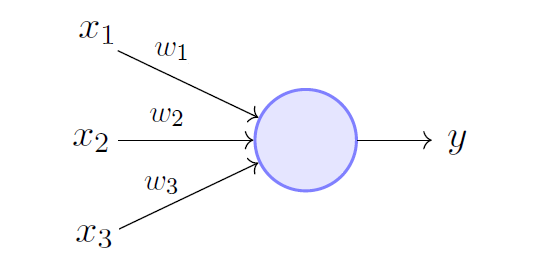
\includegraphics[scale=0.5]{perceptron2.png}
\caption{uitleg}
\label{peceptron2}
\end{figure}
\linebreak
In afbeelding \ref{peceptron2} is een perceptron te zien die 3 variabelen als input neemt: $x_{1}, x_{2}$ en $x_{3}.$ Bij all deze waardes word een gewicht(weight) toegekend($w_{n}$). Deze waarde geeft aan hoe belangrijk de input is voor deze neuron. De output van de neuron is de som van alle resultaten bij elkaar. $\sum_{j}w_{j}x_{j}$ en deze waarde vergelijken met een gekozen randwaarde(threshold) om de output the berekenen. In een meer wiskundige term:
%\begin{equation*} %tTODO write function
%\begin{rcases}
%        0  if \sum_{j}w_{j}x_{j}+b $\leq$ threshold $\\$
%        1  if \sum_{j}w_{j}x_{j}+b > threshold
%\end{rcases} 
%$\text{output}$
%\end{equation*}
 \begin{equation}
    y(x_1,\ldots,x_n) = f(w_1x_1 + w_2x_2 + \ldots + w_nx_n)  \label{per-eq}
  \end{equation}

\noindent Je kan de output van een neuron beinvloeden door te spelen met de weights en thresholds. Door een input zijn weight te vergroten of de threshold te verlagen kan er hele andere resultaten uit het model komen.\\
\newline
Het is duidelijk dat de perceptron niet een compleet model is over hoe mensen hun beslissingen nemen. Maar het voorbeeld illustreert hoe een perceptron verschillende soorten bewijs kan afwegen om beslissingen te nemen. Daarom is het aannemelijk dat een complex netwerk van perceptrons vrij subtiele beslissingen zou moeten kunnen nemen.
\begin{figure}[h!]
\centering
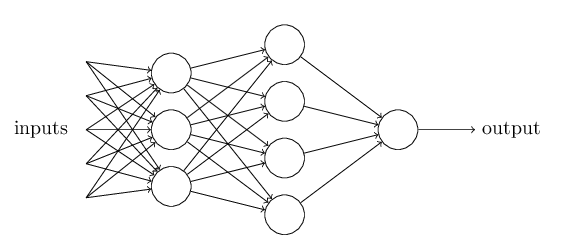
\includegraphics[scale=0.5]{perceptron3.png}
\caption{uitleg}
\label{perceptron3}
\end{figure}
\newline
In afbeelding \ref{perceptron3} is een netwerk te zien, waar de eerste laag van perceptrons in het netwerk, drie simpele beslissingen neemt door de functie in vergelijking \ref{per-eq} uit te voeren. Naast de eerste laag zit er nu ook een tweede die de outputs van de eerste laag als input neemt. Op deze manier kan een perceptron in de tweede laag een beslissing nemen op een complexer en abstracter niveau dan perceptrons in de eerste laag. Deze complexiteit en abstractheid word verhoogd per extra laag dat je toevoegd. Op deze manier kan een meerlaags netwerk van perceptrons, zeer geavanceerde beslissingen nemen.\\
\newline
De volgende stap is om ons netwerk zelf lerend te maken. Om dit te doen moet je kleine aanpassingen kunnen maken aand de weights en de biases. Deze kleine aanpassingen moet daarna ook een klein effect hebben op de output van het neurale netwerk. Echter dat is niet wat er gebeurt met perceptronen want deze heeft maar 2 outputs, een 1 en een 0. Een kleine aanpassing zal daarom niks doen of de hele uitkomst van de perceptron omdraaien. Je kan niet probleem omzeilen door een ander types neurons te gebruiken ,zoals de Sigmoid en tanh neurons.

\subsubsection{activation function}
De output van een neuron word berekend door een activation functions. Hier kijken we nu alleen naar de sigmoid en tanh activation functions want deze werken goed voor de driver. %ALLEXXXX klopt dit?
De sigmoid en tanh neurons lijken erg op perceptrons alleen de manier hoe de ouput berekend word is anders. Een sigmoid function neemt alle mogelijke nummers als een input en berekend het naar een getal tussen de 0 en 1.\\
%todo insert sigmoid
Een tanh fucntion neemt alle mogelijke nummers als input en brekend het naar en getal tussen de -1 en de 0.\\
%todo insert tanh
De twee berekeningen lijken erg op elkaar omdat tanh een scaled vorm is van de sigmoid functions.\\
omdat de data die gebruikt word voor het sturen van de torcs auto tussen de -1 en 1 zit is het verstandig om gebruik te maken van de tanh functie. Omdat tanh alle reëel getal tussen de -1 en 1 kan hebben, dus waarden zoals -0.875 ... en 0.132. Dit zorgt ervoor dat de uitkomst van een neuron niet een simple een ja of nee is maar veel complexer getal dat van alles en nog wat kan betekenen. Nu als er een kleine verandering plaatsvind in de weights of biases van het neurale netwerk zullen deze kleine verandering ook te vinden worden in de output uiteindelijk zorgt dit ervoor dat het neurale netwerk zelf kan leren.\\\\
\subparagraph{zelf lerend}
Om je netwerk wat te laten leren heb je eerst data nodig over wat je hem wil laten leren. Voor de opdracht worden er .cvs files gebruirk waar de train data van meerderen record record races op verschillende race tracks in staat.\\\\
\noindent hierna heb je een methode nodig om je neural netwerk te trainen zoals forward propagation, back propagation en resilent propagation. het doel van de algoritmns zijn om alle neurons een weight en een bias te geven. hoe dat in praktijk gaat hangt af van je dataset en welk algoritmn je gaat gebruiken maar in het kort gaat het zo:
\begin{itemize}
\item De start waarden voor je weights en biases zijn vaak random.
\item Je voert je dataset aand het network en dan krijg je daarvan de resultaten.
\item Deze resultaten vergalijk je met wat er verwacht word en je berekend het verlies.
\item Gebruik deze informatie om je netwerk bijtewerken zodat het verlies verminderd word.
\item Herhaal all deze stappen tot dat je netwerk voldoet.
\end{itemize}

\subparagraph{overfitting}
Neurale netwerken zijn erg kwetsbaar voor overfitting. Het is waar dat door meer factoren in het neurale netwerk op te nemen. Het altijd per definitie beter zal maken voor de gegevens die we al hebben ,maar een betere pasvorm voor de beschikbare gegevens betekent niet een betere voorspelling. een te eenvoudig neural netwerk maken, kan het esencetiële patroon in de data niet vastleggen. Aan de andere kant wordt een neural netwerk dat te gecompliceerd is te gevoelig voor de specifiece data die we hadden vastgelegt. Bijgevolg precies omdat het zo fijn is afgestemd op die specifieke dataset zal de oplossingen die het produceert zeer variabel zijn.\\\\


\subsection{python}

\subsection{Encog}